\documentclass[english,12pt,a4paper]{book}
\usepackage[T1]{fontenc} % In case we want special characters
\usepackage[utf8]{inputenc} % We are all writing in UTF-8

\usepackage[numbers]{natbib}
\usepackage{appendix} % Fixes formatting of appendices
\usepackage[printonlyused]{acronym} % Package to handle the acronym list
\usepackage{graphicx} % We *may* use images
\graphicspath{{images/}} % and it is clean to put them in a separate dir
\usepackage{hyperref} % Internal and external links is nice
\hypersetup{pdfborder=0 0 0} % ..especially without red borders

% Set equal margins on book style
% \usepackage{layout} % Use \layout to print out the margins (debug)
\usepackage{geometry}
\geometry{bindingoffset=1cm}

\author{Eirik Haver \and Pål Ruud}
\title{Project assignment - Tahoe-LAFS with SHA-3 candidates}
\date{\today}

\begin{document}

% Latex-versjon av ITEM rapportmal.
% Lagd av <lasse.karstensen@gmail.com>, desember 2009.
% Lisens: public domain. 
%
\begin{titlepage}
\begin{center}
\textsc{NORWEGIAN UNIVERSITY OF SCIENCE AND TECHNOLOGY\\
FACULTY OF  INFORMATION TECHNOLOGY, MATHEMATICS AND ELECTRICAL ENGINEERING} \\
\vspace{0.5cm} 
% crop-et fra http://www.ntnu.no/infoavdelingen/selvhjelp/logoer/ntnu/NTNU_engelsk_RGB.png
\includegraphics[scale=0.5]{NTNU-logo} \\

\vspace{1.0cm}
{\Huge{PROJECT ASSIGNMENT}}
\vspace{1.0cm}

\begin{tabular}{ p{4cm} p{11cm}}

Student's name:	& Eirik Haver and Pål Ruud \\
Course: & TTM13 \\
Title: & Experimenting with SHA-3 candidates in Tahoe-LAFS \\
%\vspace{1cm}
Description: & \\
\end{tabular}
{\small{\begin{tabular}{p{15cm}}
\vspace{0.2cm}
Lorem ipsum dolor sit amet, consectetur adipiscing elit. Nunc nibh quam, posuere quis dignissim vel, pulvinar vel leo. Morbi pellentesque est a magna rutrum sollicitudin. Duis nec orci porttitor tellus viverra aliquet gravida nec tellus. Aenean aliquet nulla sit amet metus sodales mattis. In pulvinar euismod consectetur. Maecenas felis nunc, suscipit ut semper et, consequat et est. 
\\\\
Donec vitae ipsum tortor. Nulla at tincidunt erat. Nunc vel risus vel mi ornare molestie non at nunc. Phasellus posuere cursus odio, nec consectetur dolor tempus quis. Proin non erat erat. Aenean et leo eros, et congue sem. Nunc auctor porta magna, ac fermentum augue malesuada vel. Nam aliquet augue eu nibh facilisis ac placerat felis vehicula. Quisque faucibus placerat vulputate. Mauris nunc turpis, venenatis ac tincidunt condimentum, tincidunt id magna. Mauris aliquet convallis accumsan. 
\\\\
\end{tabular}  }}

\begin{tabular}{ p{4cm} p{11cm}}
Deadline: & 2010-12-xx \\
Submission date: & 2010-12-xx \\
Department: & Department of Telematics \\
Supervisor: & Danilo Gligoroski \\\\
\end{tabular}
\vspace{0.5cm}

Trondheim, \today 

\vspace{0.4cm}
\line(1,0){150} \\
Danilo Gligoroski, NTNU/ITEM. 

\end{center}
\end{titlepage}


\pagestyle{empty}

\chapter*{Abstract}
\addcontentsline{toc}{chapter}{Abstract}
\pagestyle{plain}
\pagenumbering{Roman}
\setcounter{page}{1}

\chapter*{Preface}
\addcontentsline{toc}{chapter}{Preface}

\tableofcontents

\addcontentsline{toc}{chapter}{\listfigurename} % Manual, because report style
\listoffigures

\addcontentsline{toc}{chapter}{\listtablename}
\listoftables

\chapter*{Acronyms}
\addcontentsline{toc}{chapter}{Acronyms}

\begin{acronym}
\acro{AES}{Advanced Encryption Standard}
\acro{FEC}{Forward Error Correction}
\acro{LAFS}{Least-Authority Filesystem}
\acro{NIST}{National Institute of Standards and Technology}
\acro{RAM}{Random Access Memory}
\acro{SHA}{Secure Hash Algorithm}
\acro{SSE2}{Streaming SIMD Extensions 2}
\acro{SSSE3}{Supplemental Streaming SIMD Extensions 3}
\acro{SUPERCOP}{System for Unified Performance Evaluation Related to
Cryptographic Operations and Primitives}
\end{acronym}

\chapter{Introduction}
\pagenumbering{arabic}
\setcounter{page}{1}

Thorough problem description

\section{Method}

Technical procedure, Cython, two persons, test environment, how we test,
GitHub?

\section{Scope and objectives}

Should we include this?

\section{Outline}

What follows in this document, chapter by chapter


\chapter{Background technologies}
% Find new and better title

\section{Cryptographic Hash Functions}
% Get a source for this %
A Cryptographic Hash function is a deterministic mathematical procedure which
takes an arbritary block of data and outputs a fixed-size bit string. The
output is refered to as the hash value, message digest or simply digest.
Another property of a cryptographic hash function is that a small change in the
input data (just 1 bit) should completly change the output of the hash
function. In other words it should be infeasible to find the reverse of a
cryptographic hash function. It should also be infeasible to find two blocks of
data which produce the same hash value (a collision).

\subsection{NIST SHA-3 Competition}
The \ac{SHA} version 3 is a comming standard set to superceed the current
standards \ac{SHA}-1 and the \ac{SHA}-2 family. The hash function to become
\ac{SHA}-3 will be decided by \ac{NIST} and choosen between the submitted
contestants to the \ac{NIST} hash competition. The current status of the 
competition is officially called Round 2, with 14 of 64 candidates having 
survived round 1\cite{s_fedreg}. 

\subsubsection{\ac{NIST} evaluation criterias for \ac{SHA}-3}

\paragraph{Security} is the most important criteria for the SHA-3
candidates\cite{s_nistround2}. The full description of security criterias are
mentioned in \cite{s_fedreg}, however the most noteworthy criteria in regards
to Tahoe-\ac{LAFS} is that \ac{SHA}-3 candidates are required to have
resistance against length-extension attacks. Both \ac{SHA}-1 and the \ac{SHA}-2
family are vulnerable to this attack\cite{s_mdre}.

\paragraph{Cost and Performance} are considered to be the 2nd most important
criteria. The absolute minimum for performance is that the SHA-3 candidate
should be faster than the functions in the \ac{SHA}-2 family. Cost is a measure
of how much memory an implementation requires in software, both the 
implementation itself and the use of \ac{RAM} during runtime. Another measure
of cost is how many logic gates it takes to implement the function in hardware.

\paragraph{Algorithm and implementation characteristics} is the third criteria.
By this criteria \ac{NIST} emphasis that algorithms with greater flexbility
will be given preference over other algorithms\cite{s_nistround2}. By flexible
they imply the possiblity of the function to run efficiently on a varity of
plattforms, to use parallelism or instruction set extensions. Another key point
of a flexible hash function is that it should have a simple and elegant design
to encourage understanding, analysis and design confidence.

\subsection{\ac{SUPERCOP}}
% TODO: Sjekk hvordan det er med sitering her
\ac{SUPERCOP} is a toolkit developed by VAMPIRE lab for measuring performance
of cryptographic software\cite{s_supercop}. In relation to hash functions
\ac{SUPERCOP} measures the following:

\begin{itemize}
    \item Time to hash a very short packet of data
    \item Time to hash a typical-size Internet packet
    \item Time to hash a long message
    \item Length of the hash output
\end{itemize}

The round 2 \ac{SHA}-3 candidates are all included in the toolkit, with a
number of different optimalizations for each candidate. Optimalizations range
from 32-/64-bit optimalizations, the use of extended instruction sets such as
\ac{SSE2} and \ac{SSSE3}, optimalizations for different number of cores and
others. Also the toolkit will try different compiler-optimalizations to get the
best results possible for each function.
% Skal jeg sitere kildekode her?

The benchmarking results for the \ac{SUPERCOP} toolkit of \ac{SHA}-3 candidates
and \ac{SHA}-2 functions on a number of different plattforms and architectures 
are available at
\footnote{\url{http://bench.cr.yp.to/results-sha3.html}}

\section{Tahoe-LAFS}
%What is it, how/where are hash functions used, Python, pycryptopp
%comparison with RAID-6, mutable/immutable?

The Tahoe \ac{LAFS} is a system for secure,
distributed data storage. Files are encrypted client side, then
split up, before each part is sent to other nodes in the grid, as depicted in
figure \ref{fig:tahoeinsertion}. The integrity and confidentiality of the files
are guaranteed by the algorithms used on the client, and is independent of the
storage servers, which may be operated by untrusted people. This is defined as
\emph{provider-independent security} \cite{t_tahoe}.

\begin{figure}[h!]
    \centering
    \includegraphics[width=0.9\columnwidth]{Tahoe-newfile.pdf}
    \caption{Tahoe-LAFS: Insertion of new file}
    \label{fig:tahoeinsertion}
\end{figure}

Tahoe was originally developed with funding from the former commercial web
backup service provider Allmydata, but is now a stand-alone Open
Source\footnote{GNU General Public License (GPL) version 2} project
\cite{t_ars}.  It is written in the Python programming language with the Twisted
framework, and can run on Windows, Mac OSX, Linux, Solaris and more.

\subsection{Architecture}

Tahoe has a three layer architecture: the key-value store, the filesystem, and
the application.

The \textbf{key-value store}, or the ``capability-data bytes'' store, is the
lowest layer and is implemented by a grid of Tahoe-LAFS storage servers. Data is
kept on the storage servers in the form of ``shares'', which are encrypted and
encoded parts of files. Capabilities are short ASCII strings, containing
information on where to \emph{find} a file, and how to \emph{verify} it.
Nodes in the grid learn about each other through an ``introducer'', which
roughly relates to a tracker in the BitTorrent\footnote{See
\url{http://www.bittorrent.org/beps/bep\_0003.html}} protocol.

The \textbf{filesystem} layer is responsible for mapping human-meaningful
pathnames to pieces of data. Each directory contains a table of capabilities
for its children, i.e. subdirectories or files. Two forms of capabilities is
available for each file, read-only and read-write, and these can be shared to
provide shared/published directory structures with friends.

Since it is not practical for users to remember strings containing random
characters, the \textbf{application} layer is used for providing a user-friendly
interface to the directories and files.

\subsection{Related technologies}

Tahoe-\ac{LAFS} uses a number of techniques to realize the functionality
needed by a secure, distributed filesystem.

\paragraph{Erasure coding.}

When a client puts a file on the grid, it first encrypts the file, before
breaking the file into small segments. The segments are then \emph{erasure
coded}.  The use of the Solomon-Reed erasure coding scheme, enables Tahoe to
recover a file using only a predefined subset of the parts distributed to the
storage servers, i.e. the other nodes in the grid. Erasure coding is a type of
\ac{FEC} code, which extends a message with $C$ characters into a longer message
with $N$ symbols \cite{t_reed-solomon}.  The original $C$ characters can then be
recovered from a subset of the $N$ symbols.

The properties of erasure coding can be thought of as those of parity bits in
RAID\footnote{Redundant Array of Independent Disks} systems. \citet*{t_erasure}
compare erasure coding and plain replication, and conclude that ``\emph{...
erasure codes have mean time to failures many orders of magnitude higher than
replicated systems with similar storage and bandwidth requirements.}''

\paragraph{Hash Trees.}

\begin{figure}[h]
    \centering
    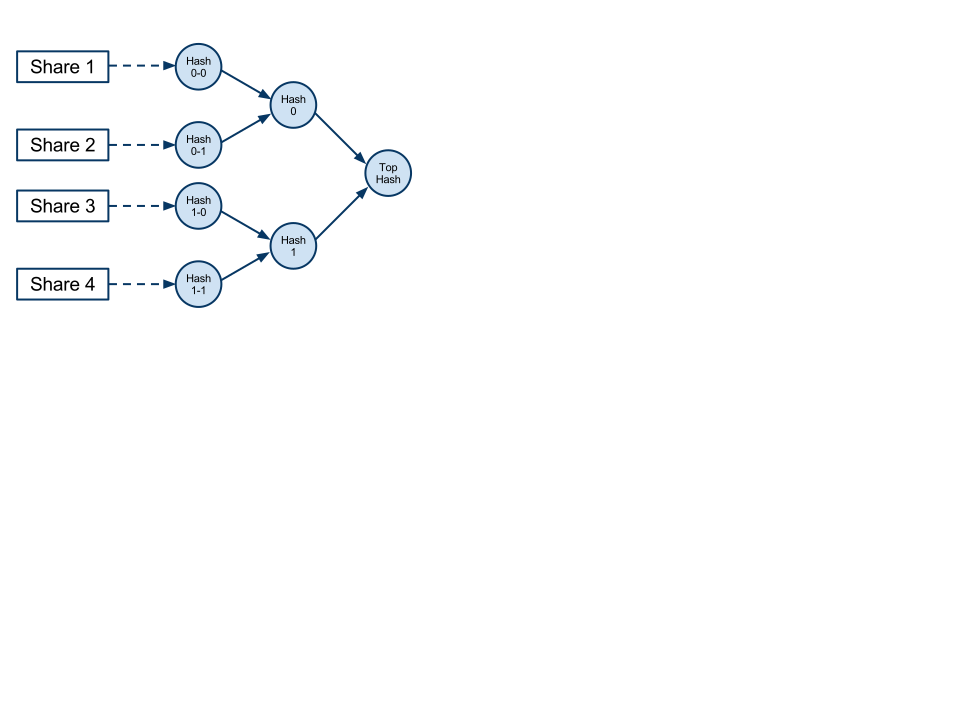
\includegraphics[width=0.9\columnwidth]{Tahoe-MerkleTree.pdf}
    \caption{Example of a Merkle tree.}
    \label{fig:tahoemerkletree}
\end{figure}

A hash tree, also known as \emph{Merkle tree}, is a type of data structure
which can be described as a tree with nodes that can verify all information
below in the hierarchy, as depicted in figure \ref{fig:tahoemerkletree}. This
enables Tahoe to verify small segments of a file at the time, and this can be
used for instance to start playing a movie file while it is still being
downloaded.


\subsection{Use of secure hashes in Tahoe-LAFS}

\begin{figure}[h]
    \centering
    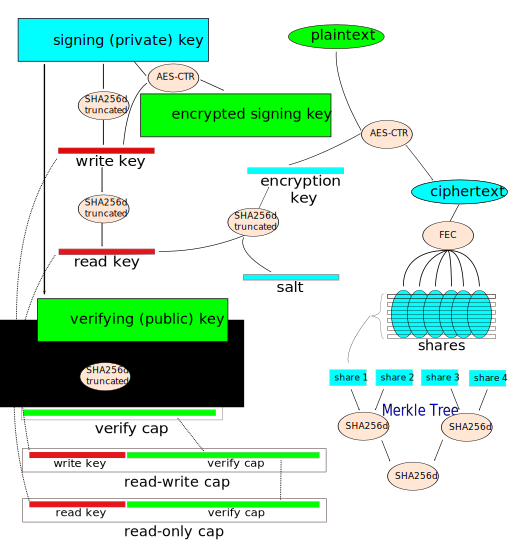
\includegraphics[width=0.9\columnwidth]{Tahoe-hashing.pdf}
    \caption{Tahoe-LAFS: Location of hashing}
    \label{fig:tahoehashing}
\end{figure}

As seen in figure \ref{fig:tahoehashing}, the usage of secure hashing is
extensive in Tahoe, and has to be considered as a key part of the functionality.


\section{Python and Cython}
%What is it, how, why, alternatives?
% TODO: Finn en kilde på pythonting, om det trengs?
Python\footnote{\url{http://www.python.org}} is a high-level general-purpose
programming language. Python is also an interpreted language, which means that
python programs are compiled at runtime.  There exists multiple implementations
of Python, however the most common, CPython, is implemented in C. The fact that
Python is a high-level language usually means that there is performance penalty
in contrast with lower level languages, shuch as C. To remedy this problem it
is possible to write extensions to the language by using the official C-API.
This approach has been used by several cryptographic libraries for python such
as the official hashlib\footnote{\url{http://code.krypto.org/python/hashlib/}}
and pycryptopp\footnote{\url{http://tahoe-lafs.org/trac/pycryptopp}}.

Tahoe-\ac{LAFS} is written in python, but the SHA-3 candidate implementations found
in both the official NIST submissions and supercop are either in C or in
assembly. Therefore it is necessary to either implement the functions in python
or make extensions to python through the C-API. Where extensions should give
the best performance. % TODO: KILDE? 

\subsection{Cython}
Cython\footnote{\url{http://www.cython.org}} is a language for writing Python
extensions in a language that closely resembles the Python language itself.
Basically what Cython does is to parse cython files and generate C source files
that utilises the Python C-API. Afterwards the generated source files can be
compiled as if they were written directly in C. A small performance tradeoff is
to be expected from this, due to the extra layer of abstraction.

\chapter{Procedure}

TODO: We have to figure out a new title
Keywords: Python bindings in detail, unit tests, using it in Tahoe-LAFS

A bit more technical description of how we tested the candidates in Tahoe-LAFS

Limitations/assumptions

Optimized candidates.

Error sources.


\chapter{Results}

What is tested and what is not tested?

tables, graphs?


\chapter{Discussion}

What could have been done differently?

Compare results with general (supercop) results.

Optimized candidates.

\cite{s_nistround2}


\chapter{Conclusion}

A somewhat short conclusion summing up results and discussion

\section{Future work}

New SHA-3 capability in Tahoe-LAFS (GSOC ref) to get our code to trunk


% BibTeX bibliography lives in external file
\bibliographystyle{plainnat}
\bibliography{ref_sha3,ref_tahoe}

\appendix
\appendixpage
\addappheadtotoc

% Use ordinary \chapters from here on..

\end{document}
